\chapter{Hierarchical Representation}\label{chp:Hierarchical Representation}
% Authors: Hongyu (Florence) Lu, Michael Gold, Erica Dominic.
% Lecture date: 1.28.19

\section{The World as a Hierarchy}
% Authors: Hongyu (Florence) Lu, Michael Gold, Erica Dominic.
% Lecture date: 1.28.19

The world is inherently compositional and hierarchical: smaller pieces combine to form larger objects.
Humans interpret the world as a hierarchy; even the visual cortex in mammals is hierarchical in nature.

The goal of deep learning is to have a machine correctly extract hierarchical representations.
Ideally, a deep neural network should detect features at one level, then detect combinations of those features at the next level.
It is important to note that not every combination of features at one level exists in the next.

\subsection{Images}
% Authors: Hongyu (Florence) Lu, Michael Gold, Erica Dominic.
% Lecture date: 1.28.19

For example, from a patch of pixels, we want to detect edges (usually by an abrupt change in color of adjacent pixels).
From edges we can discern textons (e.g. corners, crosses).
From textons we can detect motifs, then parts of objects, and finally those parts can be pieced together to detect objects within the image.

Geometrically, if we take all $5\times5$ patches of pixels in an image, we will get a collection of $25$-dimensional vectors.
These vectors, however, would likely comprise a small (low-dimensional) part of $\mathbb{R}^{25}$.

\begin{figure}[ht]
\centering
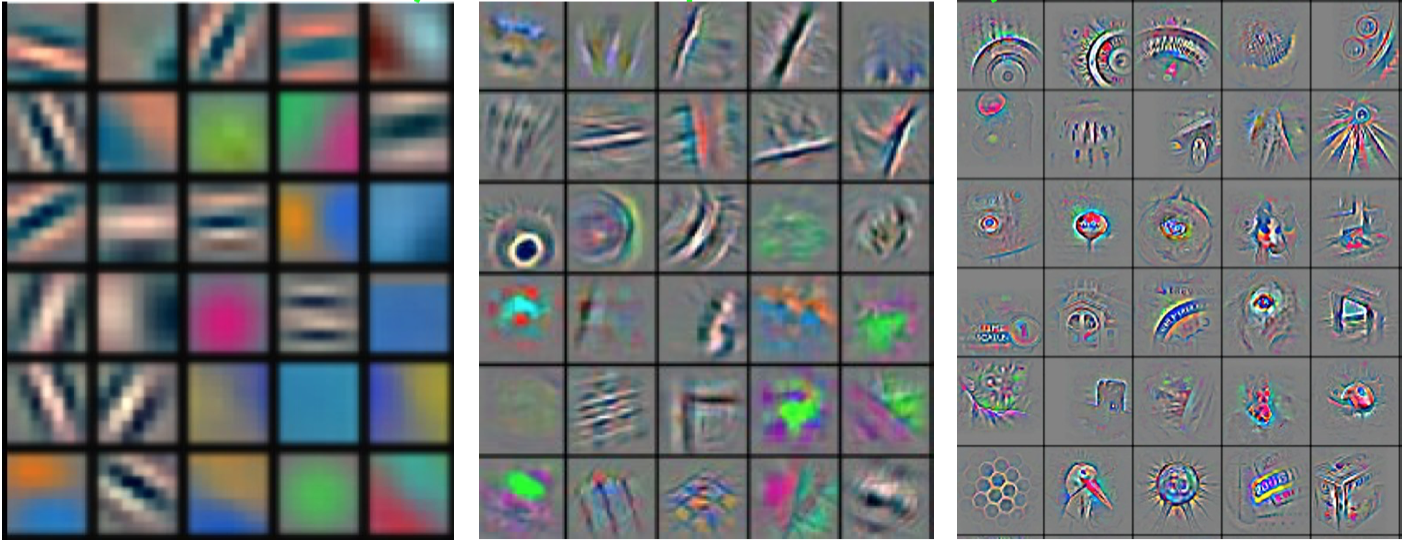
\includegraphics[width=100mm]{lectures/01-b/cnn_hierarchy.png}
\caption{Hierarchy from a convolutional neural network}
\label{fig:cnn_hierarchy}
\end{figure}

\Cref{fig:cnn_hierarchy} shows an example from a convolutional neural network.
The left pane shows detected edges, color patches, and gradients.
The middle pane has pieced those attributes together to detect textures and shapes, such as round shapes and corners.
Finally, the right pane contains discernible parts of objects.

\subsection{Text}
% Authors: Hongyu (Florence) Lu, Michael Gold, Erica Dominic.
% Lecture date: 1.28.19

The same idea can be applied to textual analysis: combinations of characters become words, combinations of words make word groups, which assemble to make clauses, which can be grouped to make sentences, and finally a collection of sentences create a story.

Again, not every combination of features at one level becomes significant in the next, e.g. not every combination of words forms a valid sentence.

\subsection{Speech}
% Authors: Hongyu (Florence) Lu, Michael Gold, Erica Dominic.
% Lecture date: 1.28.19

An audio sample is just a single number, but the frequency content of a waveform can be represented by a feature vector, and those waveforms can be pieced together to form sounds, which can then be pieced together to form syllables, etc.
Ultimately phones and phonemes are formed and pieced into words.

\chapter{Nonlinear Dimensionality Expansion}
% Authors: Hongyu (Florence) Lu, Michael Gold, Erica Dominic.
% Lecture date: 1.28.19

\section{Motivation}
% Authors: Hongyu (Florence) Lu, Michael Gold, Erica Dominic.
% Lecture date: 1.28.19

A network is ``deep'' if it has more than one stage of non-linear feature transformation. A natural question arises: why are deep networks necessary?
Theoretically, kernel machines can approximate any function with as much precision as desired.
However, that might be computationally expensive---too expensive to achieve anything in practice.

\subsection{Cover's Theorem}
% Authors: Hongyu (Florence) Lu, Michael Gold, Erica Dominic.
% Lecture date: 1.28.19

One way to rectify this problem is to bring the sample data into a higher dimension.
Thomas Cover's theorem (1965) formalized this argument.

\textbf{Cover's Theorem:} say you have a linear classifier in $N$ dimensional space with $P$ sample points, each randomly labeled with one of two class labels.
Then \cref{fig:covers_theorem} roughly illustrates the probability that these points are linearly separable.

\begin{figure}[ht]
\centering
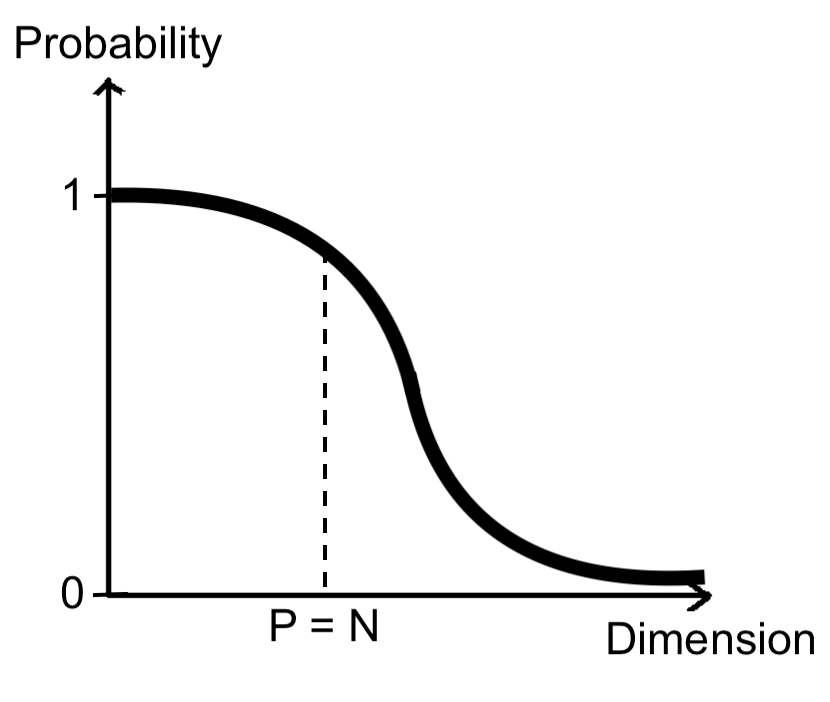
\includegraphics[width=40mm]{lectures/01-b/covers_theorem.png}
\caption{Cover's Theorem: probability of being separable vs. dimension}
\label{fig:covers_theorem}
\end{figure}

Ergo it makes sense to expand dimensionality of a representation because the data is more likely to be separable in a higher dimensional space.
One caveat: the expansion must be \emph{nonlinear}.
That brings us to deep networks, which by definition are networks with more than one nonlinear stage.

\subsection{The Manifold Hypothesis}
% Authors: Hongyu (Florence) Lu, Michael Gold, Erica Dominic.
% Lecture date: 1.28.19

Before we discuss how to expand dimensionality in a nonlinear way, we should address one concern: will working in a higher introduce an intractability problem?
The manifold hypothesis suggests that it will not pose a problem.
The manifold hypothesis postulates that natural data in high-dimensional space generally has a low-dimensional structure (see \cref{chp: manifold_hypothesis} for further discussion).
The shape of that low-dimensional space is dictated by the intrinsic factors of variation in the data, and our ideal feature extractor would extract those factors of variation.

\section{How to Expand Dimensionality Nonlinearly}\label{sec: expand_dim}
% Authors: Hongyu (Florence) Lu, Michael Gold, Erica Dominic.
% Lecture date: 1.28.19

As described in the previous section, Cover's theorem and the manifold hypothesis urge us to expand the dimension of the representation (nonlinearly) and explore it in higher dimensional space.
This is the pipeline for nonlinear dimensionality expansion:
\begin{enumerate}
    \item Linearly expand the dimension (this can be done by multiplying by matrix with more rows than columns)
    \item Apply a nonlinear transformation to each component of the vector
    \item Compress the data back into a smaller dimension (linearly or with pooling) 
\end{enumerate}

\Cref{fig:nonlinear_expansion} illustrates the process of nonlinear dimensionality expansion.
Between the first and second pane, the data is projected into higher-dimensional space linearly (observe the three-dimensional axes) and transformed nonlinearly.
Between the second and third pane, the data is brought back down to a smaller dimension (observe the two-dimensional axes) via pooling/aggregation.

\begin{figure}[ht]
\centering
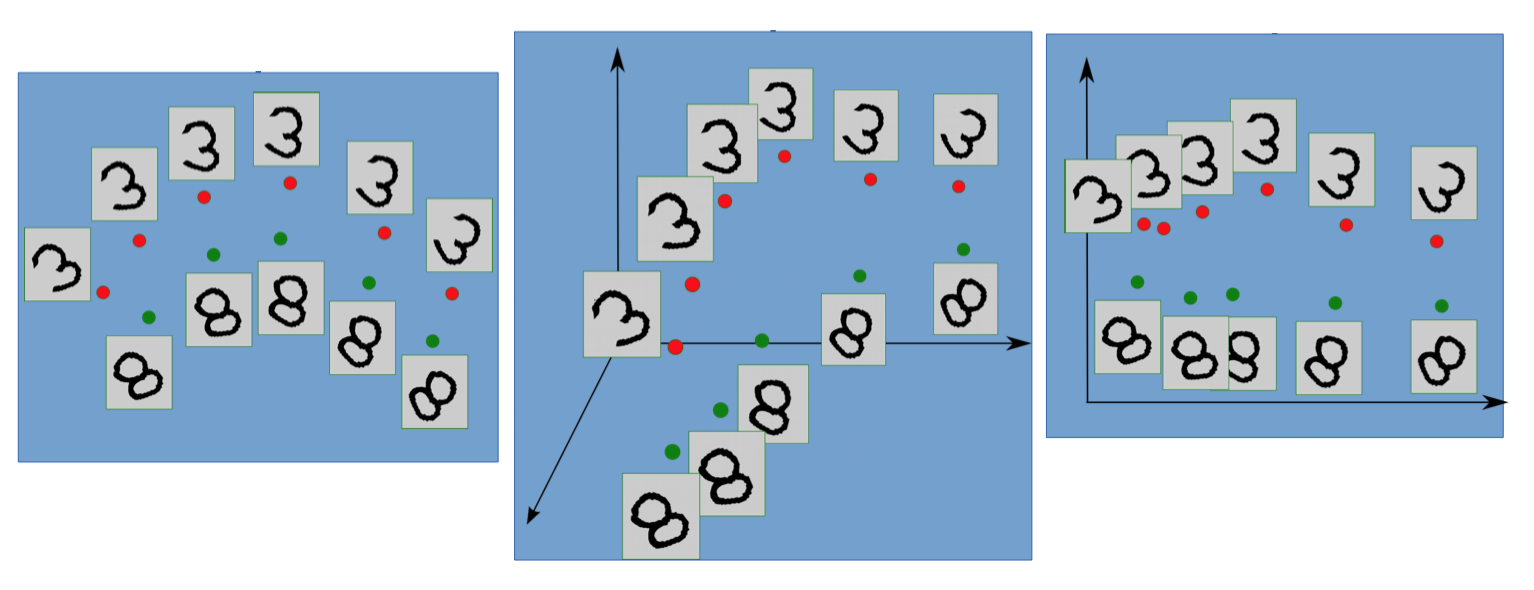
\includegraphics[width=90mm]{lectures/01-b/nonlinear_expansion.png}
\caption{Nonlinear dimensionality expansion}
\label{fig:nonlinear_expansion}
\end{figure}

\section{In the Context of the Deep Learning System Architecture}
% Authors: Hongyu (Florence) Lu, Michael Gold, Erica Dominic.
% Lecture date: 1.28.19

\Cref{sec: expand_dim} outlined the process of expanding dimensionality in a nonlinear fashion.
Here are those same steps again, this time in the context of the overall architecture for a deep learning system:
\begin{enumerate}
    \item Begin with a representation of input data
    \item Normalize the input (mean $= 0$, standard deviation $= 1$)
    \item Linearly expand the dimension (this can be done by multiplying by matrix with more rows than columns)
    \item Apply a nonlinear transformation to each component of the vector
    \item Compress the data back into a smaller dimension (linearly or with pooling) 
\end{enumerate}
This process can be repeated multiple times.

\chapter{Deep Supervised Learning: A Modular Approach}
% Authors: Hongyu (Florence) Lu, Michael Gold, Erica Dominic.
% Lecture date: 1.28.19

\section{Supervised Learning}\label{sec: supervised learning}
% Authors: Hongyu (Florence) Lu, Michael Gold, Erica Dominic.
% Lecture date: 1.28.19

\textbf{Supervised learning} is the process of improving the prediction accuracy of the outputs of some differentiable parameterized function (\textbf{module}) $G$ by learning from the discrepancies between predicted and expected outputs.
To illustrate (see \cref{fig:supervised}), suppose we would like to train a function $G(x,w)$, where $x$ is the input and $w$ is a parameter called \textbf{weight}.
Say we have an input-output pair $(x,y)$.
The function $G(x,w)$ first takes the input $x$ and predicts an output $\bar{y}$.
Then, the \textbf{cost function} $C(\bar{y},y)$ measures the distance between the expected output $\bar{y}$ and the predicted output $\bar{y}$ and returns a \textbf{cost}, that is, a scalar value indicating the error in prediction.
Finally, the weight $w$ will be adjusted according to the cost by using a method called \textbf{stochastic gradient descent}. 

Some examples of modules can be found in \cref{ssc:Module Classes}. 

\begin{figure}[ht]
\centering
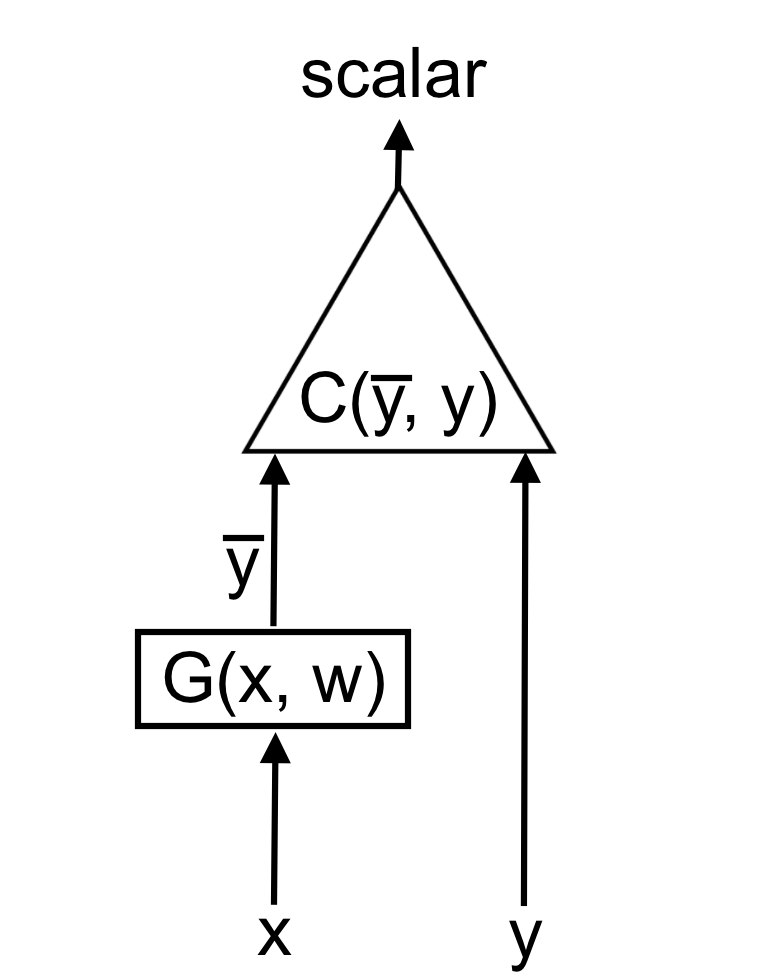
\includegraphics[width=30mm]{lectures/01-b/supervised.png}
\caption{Supervised learning}
\label{fig:supervised}
\end{figure}

\section{Stochastic Gradient Descent}\label{sec: SGD}
% Authors: Hongyu (Florence) Lu, Michael Gold, Erica Dominic.
% Lecture date: 1.28.19

Suppose we are given a training data set consisting of $P$ pairs of inputs and their associated outputs $(x^i, y^i)$, where $i \in [1, P]$.
We would like to optimize the weights $\vect{w}$ of some function according to the error produced by an objective function:
\[
L(x^i, y^i, \vect{w}) = C(G(x^i, \vect{w}), y^i).
\]
Recall that \textbf{gradient descent} calculates the derivative of the cost function in attempt to find the minimal cost.
If we compute the gradient for the entire training set, it may be too computationally expensive for very large training sets.
Instead, a more efficient method is adopted called \textbf{stochastic gradient descent}.
This method evaluates the gradient randomly at the $i^\text{th}$ pair of input and output, and the weight vector $\vect{w}$ is immediately updated accordingly for each iteration with a learning rate $\eta$:
\begin{equation}\label{eq: SGD}
\vect{w} \leftarrow \vect{w} - \eta \left[ \frac{\partial L(x^i, y^i, \vect{w})}{\partial \vect{w}} \right]^\top
\end{equation}
Note that $\vect{w}$ is a vector which has the same dimension as the input $x^{i}$.
The result is a row vector consisting of partial derivatives with respect to each component of $\vect{w}$:
\[
\left[ \frac{\partial L(x^i, y^i, \vect{w})}{\partial \vect{w}} \right]^\top = \left[ \hspace{2mm} \frac{\partial L}{\partial w_1} \hspace{2mm} \frac{\partial L}{\partial w_2} \hspace{2mm} \cdots \hspace{2mm} \right]
\]
These partial derivatives are then evaluated using a method called \textbf{backpropagation}, which will be introduced in \cref{ssc: Compute SGD using backprop}.

\section{Multi-layer Neural Network}\label{sec: Systems with Multiple Modules}
% Authors: Hongyu (Florence) Lu, Michael Gold, Erica Dominic.
% Lecture date: 1.28.19

The above supervised learning algorithm uses only one module to predict the output $\bar{y}$.
Often, we can build a complex learning machine by assembling modules into networks.
\Cref{fig: multimodule_cascade} illustrates a simple example of a multimodule system.
This system has a \textit{cascade}, or \textit{sequential}, architecture, that is, a structure where no cycles are formed in the network and the input $X$ is passed forward in only one direction.
We can use a recurrence equation to represent a system with $n$ modules:
\[
X_i = F_i(X_{i-1}, W_i)
\]
for all $i \in [1, n]$.
Here, each module $F_i$ is an object that contains trainable parameters $W_i$.
The output of the $(i-1)^\text{th}$ module $X_{i-1}$ is returned and stored internally.
It is then taken as the input for the $i^\text{th}$ module $F_i$ and so on until the signal reaches the last module $F_n$ and computes the predicted output $X_n$.

\begin{figure}[ht]
\centering
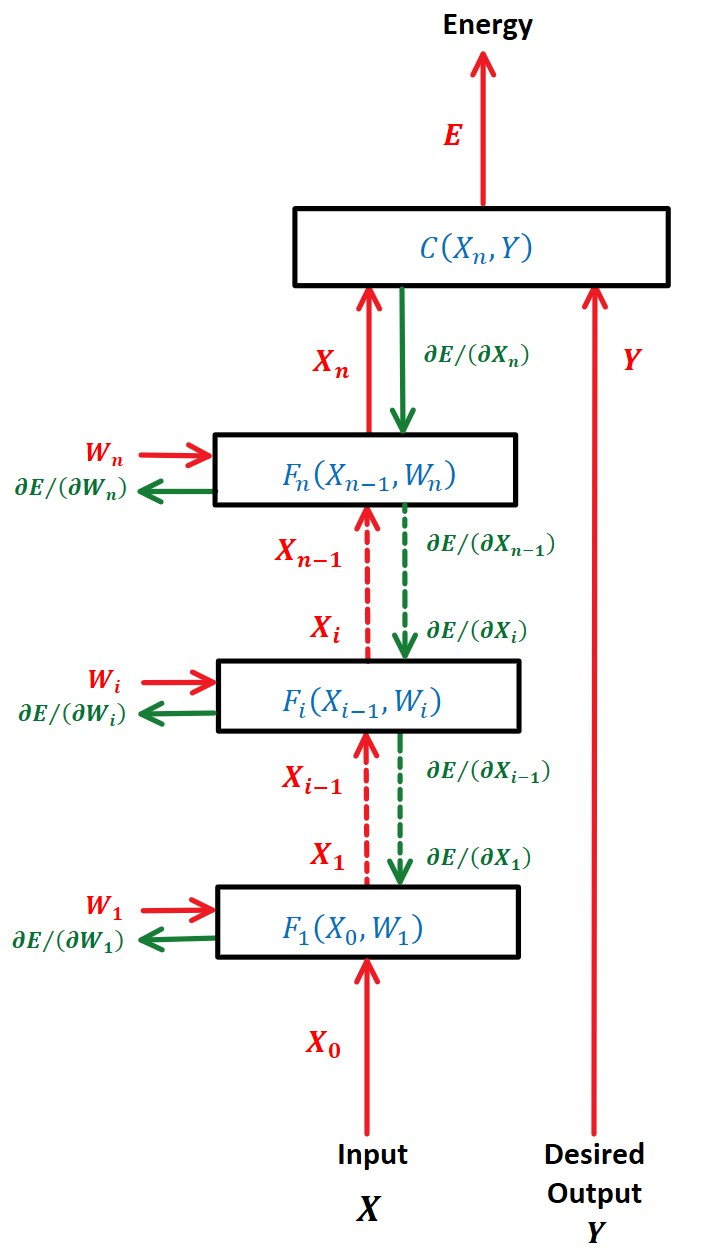
\includegraphics[width=70mm]{lectures/01-b/multimodule_cascade.jpg}
\caption{Multimodule cascade/sequential system}
\label{fig: multimodule_cascade}
\end{figure}

Similar to a single module system, the objective function $E$ that we would like to optimize is the cost function:
\[
E(Y, X_0, W) = C(X_n, Y)
\]
which measures the distance between the predicted output $X_n$ of and the desired output $Y$. 
\section{Backpropagation}\label{sec: Backpropagation}
% Authors: Hongyu (Florence) Lu, Michael Gold, Erica Dominic.
% Lecture date: 1.28.19

Recall that a learning algorithm is considered ``deep'' if it has more than one layer.
A multimodule system with a sequential structure is often called a \textbf{multi-layer feedforward neural network}, or a \textbf{deep neural network}.
See an example of defining a two-layer neural network in PyTorch in \cref{sec: Multilayer Neural Network}.
In PyTorch, as the signal of the initial input $X_0$ propagates through a sequence of approximation functions $F_i$, PyTorch instantaneously generates another function internally, called \textbf{backpropagation}, that propagates the cascade of modules backwards in order to compute gradients discussed in \cref{sec: SGD}. 

\subsection{Compute Gradient Using Backpropagation}\label{ssc: Compute SGD using backprop}
% Authors: Hongyu (Florence) Lu, Michael Gold, Erica Dominic.
% Lecture date: 1.28.19

To compute the gradient of the objective function $E(W,Y,X)$ in an $n$-layer neural network, first consider a module $F_k$ in the network, where $k\in (0, n)$.
The forward propagation method uses the input $X_{k-1}$ produced by the $(k-1)^{\text{th}}$ module and computes a predicted output $X_k$ using the weight $W_k$, 
\[ X_k=F_k(X_{k-1},W_k). \]
Suppose we know the gradient $\frac{\partial E}{\partial X_k}$ of the cost function with respect to the output of the $k^\text{th}$ module.
That is, for each component of the vector $X_k$, we know how much $E$ wiggles if we wiggle that component of $X_k$.
As mentioned in \cref{sec: supervised learning}, since the goal is to adjust the weight $W_k$, we would like to know how much $E$ wiggles if wiggle each component of $W_k$, namely, the gradient $\frac{\partial E}{\partial W_k}$ of the cost function with respect to the weight of the $k^\text{th}$ module.
To do so, we can simply apply the chain rule using $\frac{\partial E}{\partial X_k}$: 
\[
\frac{\partial E}{\partial W_k} = \frac{\partial E}{\partial X_k} \frac{\partial F_k(X_{k-1},W_k)}{\partial W_k}.
\]
In particular, each element $(p,q)$ of the Jacobian matrix indicates how much the $p^\text{th}$ output wiggles when we wiggle the $q^\text{th}$ weight:
\[
\left[ \frac{\partial F_k(X_{k-1},W_k)}{\partial W_k} \right]_{pq} = \frac{[\partial F_k(X_{k-1},W_k)]_p}{\partial [W_k]_q}.
\]
Then, using the same method, we compute the gradient $\frac{\partial E}{\partial X_{k-1}}$ of the cost function with respect to the input of the $k^\text{th}$ module in order to pass the signal to the $(k-1)^\text{th}$ module for it to repeat the above process again.
A chain rule is applied:
\[
\frac{\partial E}{\partial X_{k-1}} = \frac{\partial E}{\partial X_k} \frac{\partial F_k(X_{k-1},W_k)}{\partial X_{k-1}}.
\]
Note that 
\[
\frac{\partial F_k(X_{k-1},W_k)}{\partial W_k}, \frac{\partial F_k(X_{k-1},W_k)}{\partial X_{k-1}}
\]
are the \textbf{Jacobian matrices} of the module $F_k$ with respect to  $W_k$ and $X_{k-1}$.

The entire process of recursively calculating gradients $\frac{\partial E}{\partial X_{i-1}}$ and $\frac{\partial E}{\partial W_i}$ starting from the $n^\text{th}$ module backwards to the first module in the network is called \textbf{backpropagation}.
We have (see \cref{fig: multimodule_cascade}),

\begin{align*}
 \frac{\partial E}{\partial X_n} &= \frac{\partial C(X_n, Y)}{\partial X_n}\\
 \frac{\partial E}{\partial X_{n-1}} &=\frac{\partial E}{\partial X_n} \frac{\partial F_n(X_{n-1},W_n)}{\partial X_{n-1}} \\  
 \frac{\partial E}{\partial W_n} &=\frac{\partial E}{\partial X_n} \frac{\partial F_n(X_{n-1},W_n)}{\partial W_n} \\
 &\vdots\\ 
 \frac{\partial E}{\partial X_{i-1}} &=\frac{\partial E}{\partial X_i} \frac{\partial F_n(X_{i-1},W_i)}{\partial X_{i-1}} \\  
 \frac{\partial E}{\partial W_i} &=\frac{\partial E}{\partial X_i} \frac{\partial F_i(X_{i-1},W_i)}{\partial W_i} \\
   &\vdots\\ 
 \frac{\partial E}{\partial X_0} &=\frac{\partial E}{\partial X_1} \frac{\partial F_n(X_0,W_1)}{\partial X_0} \\  
 \frac{\partial E}{\partial W_1} &=\frac{\partial E}{\partial X_1} \frac{\partial F_1(X_0,W_1)}{\partial W_1} \\
\end{align*}

\subsection{Some Module Classes}\label{ssc:Module Classes}
% Authors: Hongyu (Florence) Lu, Michael Gold, Erica Dominic.
% Lecture date: 1.28.19

Several module classes are discussed here along with their respective gradients as they are the most commonly used modules to build a multi-layer neural network.

\textbf{Cost module}.
A typical cost module is a squared distance function $C=\|\bar{Y}-Y\|^2$ which measures the distance between predicted and expected outputs.
It is mostly used to indicate errors in prediction.

\textbf{Linear module}.
A linear module is a function $Y=W\cdot X$ that predicts an output $Y$ by multiplying a Jacobian matrix $W$ by the input $X$.
The gradients of the cost function with respect to input and weight are 
\begin{align*}
    \frac{\partial C}{\partial X} &= W^\top \cdot \frac{\partial C}{\partial Y} \\
    \frac{\partial C}{\partial W} &= W^\top \cdot \frac{\partial C}{\partial Y} 
\end{align*}
respectively.

\textbf{ReLU module}.
A Rectifier Linear Unit(ReLU) is a pointwise nonlinearity $Y=ReLU(X)$ which takes an input $X$ and returns the identity function $Y=X$ if $X>=0$ and $0$ if $X<0$.
The gradient is 
\begin{equation}
    \frac{\partial C}{\partial X} =
    \begin{cases}
     \frac{\partial C}{\partial Y}, &\text{if } X\geq 0 \\
      0 , &\text{otherwise}
    \end{cases}
\end{equation}

\textbf{Duplicate module}.
A duplicate module $Y_1=X, Y_2=X$ makes two copies of the input $X$ and return two identical outputs $Y_1$ and $Y_2$.
The gradient with respect to the input for this module is 
\[
\frac{\partial C}{\partial X} = \frac{\partial C}{\partial Y_1} + \frac{\partial C}{\partial Y_2}
\]
since two costs are adjusted when we adjust the weight of the function.

\textbf{Add module}.
An add module $Y=X_1+X_2$ is a simple addition on two inputs $X_1$ and $X_2$.
If we adjust the weight of the function, only one cost will be adjusted.
Therefore, the gradients of the inputs are the same
\[
\frac{\partial C}{\partial X_1} = \frac{\partial C}{\partial Y} = \frac{\partial C}{\partial X_2}
\]

\textbf{Max module}.
A max module $Y=\max(X_1,X_2)$ compares the first input $X_1$ to the second input $X_2$ and returns the identity function if $X_1>X_2$ and $0$ otherwise.
Since the value of of $X_2$ is never passed forward, gradient of the input is only calculated with respect to $X_1$, that is,

\begin{equation}
    \frac{\partial C}{\partial X_1} =
    \begin{cases}
     \frac{\partial C}{\partial Y}, &\text{if } X_1 > X_2 \\
      0 , &\text{otherwise}
    \end{cases}
\end{equation}

\textbf{LogSoftMax module}.
A LogSoftMax module given by
\[
Y=\log\left(\frac{\exp{(X)}}{\sum_j\exp{(X_j)}}\right) = X - \log\left(\sum_j\exp{(X_j)}\right)
\]
normalizes the given input $X$ to a probability distribution indicating the likelihood in $[0,1]$.
The gradient is computed as follows:
\[
\frac{\partial C}{\partial X} = 1 -  \frac{\exp{X}}{\sum_j\exp{(X_j)}}
\]
Note that the sum of all components $X_j$ of an input $X$ is equal to $1$.